
\documentclass[12pt,article]{memoir}

\usepackage{fancyhdr}
\usepackage{graphicx}
\usepackage{fontspec}
\setmainfont{Calibri}
\usepackage{tikz}
\usetikzlibrary{calc}
\usepackage{xcolor}
\usepackage{xpatch}
\usepackage{hyperref}

\usepackage{fancyhdr}
\usepackage{graphicx}
\usepackage{fontspec}
\setmainfont{Calibri}
\usepackage{tikz}
\usetikzlibrary{calc}
\usepackage{xcolor}
\usepackage{xpatch}
\usepackage{hyperref}
\usepackage{tabu}
\usepackage{float}
\usepackage[autostyle, english = american]{csquotes}


\usepackage[yyyymmdd]{datetime} % change date format to yyyy/mm/dd to fit ISO8601

\renewcommand{\familydefault}{\sfdefault} % set font
\renewcommand{\dateseparator}{--} % change date-seperators to - to fit ISO8601

\renewcommand\contentsname{Table of Contents}

\chapterstyle{section}
\renewcommand*{\chapnumfont}{\normalfont\HUGE\bfseries\sffamily}
\renewcommand*{\chaptitlefont}{\normalfont\HUGE\bfseries\sffamily}

\makeatletter 
% define macro for itemcode
\newcommand\itemcode[1]{\renewcommand\@itemcode{#1}}
\newcommand\@itemcode{}

% define macro for rev number
\newcommand\revnumber[1]{\renewcommand\@revnumber{#1}}
\newcommand\@revnumber{}
\makeatother

\definecolor{orbitOrange}{RGB}{250,62,0} % the ORBiT orange

\setlrmarginsandblock{2.5cm}{2.5cm}{*}
\setulmarginsandblock{2.5cm}{*}{1}
\checkandfixthelayout 

\setlength{\beforechapskip}{0cm} % reduce chapter spacing

\hypersetup{
    colorlinks,
    citecolor=black,
    filecolor=black,
    linkcolor=black,
    urlcolor=black
}

%**********************************************************************
%Document titles etc. defined here: (replace [] as well)
\title{ORBiT Avionics II System Requirement}
\author{Jinzhi Cai}
\itemcode{Sys-Req}
\revnumber{A01}
\date{\today}
%end of document titles etc.
%**********************************************************************

\makeatletter
\let\runtitle\@title
\let\runitemcode\@itemcode
\makeatother

% set header style
\pagestyle{fancy}
{
	\fancyheadoffset{0cm}

	\lhead{\runtitle \ - \runitemcode}
	\rhead{Page: \thepage }
	%\chead{\leftmark} % section name
}

\newcommand{\OrbitBackground}{% For a logo drawn with TikZ
\begin{tikzpicture}[remember picture,overlay] % draw background
	\coordinate (bl) at (current page.south west);
	\coordinate (r) at (current page.east);
    \coordinate (A) at ($(bl)+(0,3cm)$);
    \coordinate (B) at ($(r)+(0,-2cm)$);
    \coordinate (C) at (current page.south east);
    \coordinate (ctrlNode) at ($(current page.south) + (0cm,1cm)$);
    \coordinate (ctrlNode2) at ($(current page.south east) + (-1cm,1cm)$);
    \fill[orbitOrange, fill opacity=0.2]
    (A) .. controls (ctrlNode) and (ctrlNode2) .. (B) -- (C) -- (bl);
    \node [white] at ($(C) + (-3cm,1cm)$) {2015-\the\year \ ORBiT@SU};
\end{tikzpicture}
}

\cfoot{\OrbitBackground}

\begin{document}

\begin{tikzpicture}[remember picture,overlay] % draw background
	\coordinate (bl) at (current page.south west);
	\coordinate (r) at (current page.east);
    \coordinate (A) at ($(bl)+(0,3cm)$);
    \coordinate (B) at ($(r)+(0,-2cm)$);
    \coordinate (C) at (current page.south east);
    \coordinate (ctrlNode) at ($(current page.south) + (0cm,1cm)$);
    \coordinate (ctrlNode2) at ($(current page.south east) + (-1cm,1cm)$);
    \fill[orbitOrange]
    (A) .. controls (ctrlNode) and (ctrlNode2) .. (B) -- (C) -- (bl);
    \node [white] at ($(C) + (-3cm,1cm)$) {2015-\the\year \ ORBiT@SU};
\end{tikzpicture}

\makeatletter
	
\includegraphics[width=\textwidth]{../logo.jpg}\\[4ex]
	\begin{center}
	{\fontsize{50}{60}\selectfont \bfseries  \@title }\\[2ex] 
	{\LARGE  \@itemcode}\\
	\end{center}
	\begin{flushright}
	\vspace*{\fill}
	{\LARGE Rev: \@revnumber}\\[2ex]
	{\large \@author}\\[2ex]
	{\large \@date}\\[20ex]
	\end{flushright}
\makeatother
\thispagestyle{empty}
\newpage

\tableofcontents*
\thispagestyle{fancy}
\newpage

%**********************************************************************
% Everything after this is the main document. Edit below this line,

\chapter{Introduction to ORBiT Avionics II System (OA-II)}
\section{Introduction}
ORBiT Avionics II System is a new generation avionics system for Orange Rocket Ballistics Team rocket. It include twq major part, the On Board part, and the Base Station part. All the compone in the OA-II system are inter connect with a unique backplane system and wireless system.
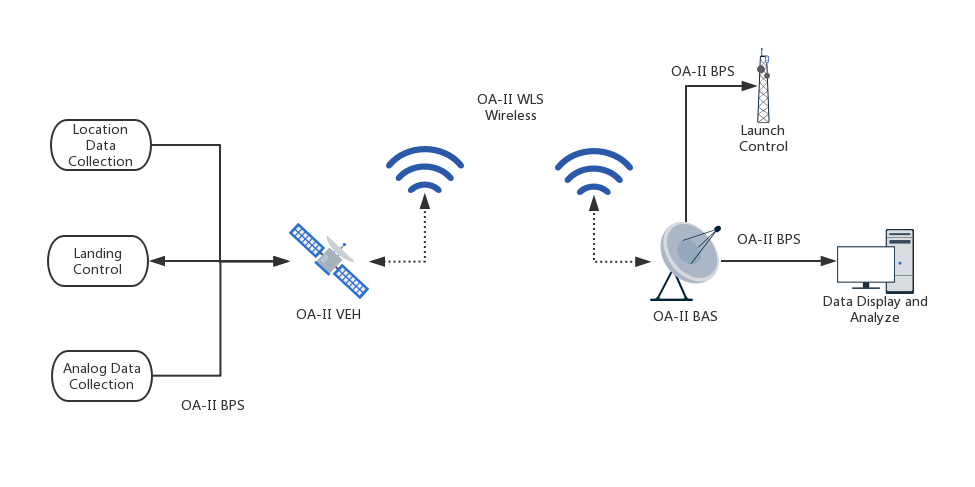
\includegraphics[width=\textwidth]{sys_diag.png}
\subsection{On Board Part (OBP)}
The OA-II OBP is use to collecting information about the rocket and deliver it to the OA-II BSP for further analysis. In the same time, it also will back up all the information to a on board storage in case wireless connection failure.
\subsection{Base Station Part (BSP)}
The OA-II BSP is use to receive the information delivered by OA-II OBP via wireless connection and perform basic analyze on roket status. The OA-II BSP provide live for rocket status and location and data storage for further analysis. The OA-II BSP also help to indetify the rocket location after it is landed for reclaim personnel to locate the rocket.
\subsection{Backplane System (BPS)}
The OA-II BPS is a unique, muti-level information exchange system that link different part in the OA-II BSP and the OA-II OBP. It provide different speed mode for different compone.
\subsection{Wireless System (WLS)}
The OA-II WLS is a wireless communication system which provide communication between OA-II BPS and OA-II OBP. In the same time, it also provide landing locating signal.
\section{Requirement}
\subsection{On Board Part (OBP)}
Reqire feature
\begin{itemize}
\item Three dimension linear kinematics data. P(position), V(velocity), A(acceleration) data.
\item Three dimension Rotational kinematics data. \theta(angle), \omega(angular velocity), \alpha(angular acceleration) data.
\item Air pressure data.
\item Sound frequency level ADC(Sample frequency \geq 40kHz)
\item Power manage (convert from 24V)
\item High power driver (Peak Power \geq 50W)
\item 720p 24Hz RGB Camera 
\item Landing location broadcast (up to 2 hours, 3km range, low power consumption)
\end{itemize}
Addtional feature
\begin{itemize}
\item Radio frequency level ADC(Sample frequency \geq 4GHz)
\item 1080p 60Hz RGB Camera 
\end{itemize}
\subsection{Base Station Part (BSP)}
Reqire feature
\begin{itemize}
\item Receving Data from rocket.
\item Display Rocket Status informaiton.
\item Basic Data analyzation(Normal/Warning/Error Status).
\item Locate rocket after landing.
\item Ignition control system\\
Rocket engine fual injection and ignition\\
Critical cutoff\\
Fire control\\
\end{itemize}
Addtional feature
\begin{itemize}
\item Rocket Tracking(via camera or radio)
\item Launch Pad Control
\item Automatic system check
\end{itemize}
\subsection{Backplane System (BPS)}
\begin{itemize}
\item Provide different speed mode with ms level delay \\
Info level( \leq 3MB/s)\\
Data level(\approx 50MB/s)\\
Stream level(\geq 100MB/s)
\item Tolerance high vibration and EMP
\item Tolerance high temperture (\leq $75^{\circ}C$)
\end{itemize}
\subsection{Wireless System (WLS)}
\begin{itemize}
\item Provide high speed data connection within 10km
\item Provide low speed, low power consumption data connection within 3km
\end{itemize}
\chapter{Revision History}
\begin{table}[H]
	\centering
	\begin{tabu}{r || c | c | c }
		Reversion Number & Person & Change Log & Time\\ \hline
		A01 & Jinzhi Cai & Initialize  & 2019-6-21 \\
		 & & & \\
		 & & & \\
		 & & & \\
		 & & & \\
	\end{tabu}
	\caption{Summary of Revision History}
	\label{tab:edatools}
\end{table}

%end of document
%**********************************************************************
\end{document}